% ===========================================================================
\chapter{Proposed Methodology}
% ===========================================================================

\section{System Architecture}

The proposed framework is an intelligent Deep Reinforcement Learning system for security posture aware SFC placement. It consists of five principal components, as illustrated in Figure~\ref{fig:architecture}:

\begin{enumerate}
  \item \textbf{Substrate Network}: a dynamic graph whose node resources, link bandwidths, and security posture states evolve as VNFs are allocated, expire, and security incidents occur.
  \item \textbf{SFC Request Generator}: produces incoming SFC requests with random VNF demands and constraints.
  \item \textbf{SFC Placement Environment}: a Gymnasium-compatible MDP environment implementing the state, action, security posture-aware reward, and constraint logic.
  \item \textbf{Maskable PPO Agent}: the DRL backbone that trains on rollouts collected from the environment, updating its policy and value networks using the PPO objective.
  \item \textbf{GNN Feature Extractor}: encodes the substrate topology and node states — including current security posture — into rich embeddings for the DRL policy network.
\end{enumerate}

\begin{figure}[!ht]
\centering
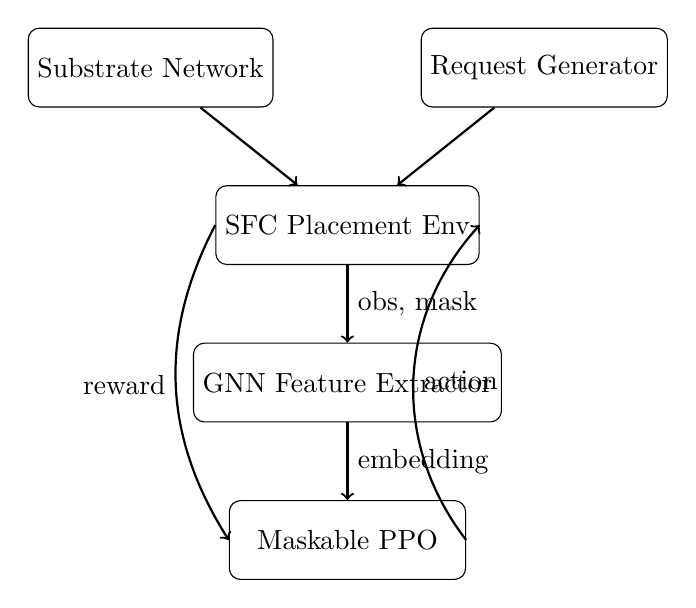
\begin{tikzpicture}[
  box/.style={rectangle, draw, rounded corners, minimum width=3cm, minimum height=1cm, text centered},
  arrow/.style={->, thick}
]
\node[box] (sub) at (0,0) {Substrate Network};
\node[box] (gen) at (5,0) {Request Generator};
\node[box] (env) at (2.5,-2) {SFC Placement Env};
\node[box] (gnn) at (2.5,-4) {GNN Feature Extractor};
\node[box] (ppo) at (2.5,-6) {Maskable PPO};

\draw[arrow] (sub) -- (env);
\draw[arrow] (gen) -- (env);
\draw[arrow] (env) -- node[right]{obs, mask} (gnn);
\draw[arrow] (gnn) -- node[right]{embedding} (ppo);
\draw[arrow] (ppo.east) to[bend left=40] node[right]{action} (env.east);
\draw[arrow] (env.west) to[bend right=30] node[left]{reward} (ppo.west);
\end{tikzpicture}
\caption{High-level system architecture of the proposed framework.}
\label{fig:architecture}
\end{figure}

\section{Maskable Proximal Policy Optimization as the DRL Backbone}

\subsection{PPO Background}

Proximal Policy Optimization (PPO) \cite{schulman2017} is the Deep Reinforcement Learning algorithm used as the backbone of our framework. It optimizes the following surrogate objective:
\begin{equation}
L^{\text{CLIP}}(\theta) = \mathbb{E}_t\!\left[\min\!\left(r_t(\theta)\hat{A}_t,\; \text{clip}(r_t(\theta), 1-\epsilon, 1+\epsilon)\hat{A}_t\right)\right],
\end{equation}
where $r_t(\theta) = \pi_\theta(a_t \mid s_t) / \pi_{\theta_{\text{old}}}(a_t \mid s_t)$ is the probability ratio, $\hat{A}_t$ is the Generalized Advantage Estimate (GAE) \cite{schulman2016}, and $\epsilon = 0.2$ is the clipping range. The full PPO loss also includes an entropy bonus $H[\pi_\theta(s_t)]$ (coefficient $c_e = 0.01$) and a value function loss (coefficient 0.5).

GAE with parameter $\lambda_{\text{GAE}} = 0.97$ is used to estimate advantages, balancing bias and variance:
\begin{equation}
\hat{A}_t = \sum_{l=0}^{T-t-1} (\gamma \lambda_{\text{GAE}})^l \delta_{t+l},
\end{equation}
where $\delta_t = r_t + \gamma V(s_{t+1}) - V(s_t)$ is the TD residual.

\subsection{Maskable PPO Extension}

Maskable PPO \cite{sb3contrib2021} extends the standard PPO DRL algorithm by accepting a binary action mask $\mathbf{m}_t \in \{0,1\}^{|\mathcal{A}|}$ at each step. The policy is defined as:
\begin{equation}
\pi_\theta(a \mid s_t) = \frac{\exp(z_a) \cdot m_a}{\sum_{a'} \exp(z_{a'}) \cdot m_{a'}},
\end{equation}
where $z_a$ are the raw logits from the policy network and $m_a \in \{0,1\}$ is the mask. In practice, this is implemented by replacing logits of masked actions with $-10^8$ before applying softmax.

The key implication is that infeasible actions have zero probability under the policy for all time, guaranteeing that the agent never selects a constraint-violating node — including nodes that fail the security posture constraint. This is in contrast to soft constraint methods, where infeasible actions are penalized but not forbidden.

\subsection{Training Configuration}

Table~\ref{tab:training} summarizes the training hyperparameters used in our experiments.

\begin{table}[!ht]
\centering
\caption{Maskable PPO Training Hyperparameters}
\label{tab:training}
\begin{tabularx}{\textwidth}{X X X}
\hline
\textbf{Hyperparameter} & \textbf{Value} & \textbf{Description} \\ \hline
Total timesteps & 100,000 & Total environment steps \\
$n_{\text{steps}}$ & 4,096 & Steps per rollout collection \\
Batch size & 512 & Mini-batch size for updates \\
$n_{\text{epochs}}$ & 10 & Update epochs per rollout \\
Learning rate & $10^{-4}$ & Constant learning rate \\
Discount factor $\gamma$ & 0.99 & Reward discount \\
GAE $\lambda$ & 0.97 & Advantage estimation parameter \\
Clip range $\epsilon$ & 0.2 & PPO clipping parameter \\
Entropy coefficient $c_e$ & 0.01 & Entropy bonus \\
Episode length $T$ & 300 & Requests per episode \\
Risk penalty $\lambda$ & 4.0 & Risk-reward coefficient \\
AR window $w$ & 10 & Windowed acceptance ratio size \\
AR weight $\omega$ & 0.5 & AR modifier weight \\
\hline
\end{tabularx}
\end{table}

\section{GNN Feature Extractor}

\subsection{Architecture Overview}

The GNN Feature Extractor (`GNNFeaturesExtractor`) is embedded within the DRL policy network as a Stable-Baselines3 `BaseFeaturesExtractor` \cite{raffin2021}. It processes the Dict observation $({\mathbf{F}},\; \mathbf{g},\; \mathbf{m}^P,\; \mathbf{m}^N)$ — which includes each node's current security posture in the node feature matrix — and produces a fixed-dimensional feature vector $\mathbf{e} \in \mathbb{R}^{d_f}$ (with $d_f = 256$) that is fed into the actor-critic MLP heads.

The forward pass proceeds in four stages:

\begin{enumerate}
  \item \textbf{Node feature preparation:} Node features $\mathbf{F} \in \mathbb{R}^{N \times 6}$ and placement mask $\mathbf{m}^P \in \mathbb{R}^N$ are concatenated to form the input $\mathbf{X} \in \mathbb{R}^{N \times 7}$.
  \item \textbf{GNN message passing:} Multiple GNN layers propagate information across the substrate graph, producing node embeddings $\mathbf{H} \in \mathbb{R}^{N \times d_h}$ (with $d_h = 64$).
  \item \textbf{Attention-weighted aggregation:} A learned attention network produces a graph-level embedding $\mathbf{e}^G \in \mathbb{R}^{d_h}$.
  \item \textbf{Global context fusion:} The graph embedding is concatenated with the processed global context $\mathbf{e}^C \in \mathbb{R}^{64}$ and passed through a fusion MLP to produce $\mathbf{e} \in \mathbb{R}^{d_f}$.
\end{enumerate}

\subsection{GNN Layer Configurations}

Three GNN architectures are supported:

\textbf{GCN} \cite{kipf2017}: three `GCNConv` layers with input dimension 7 and hidden dimension 64, each followed by LayerNorm and ReLU. Dropout (0.1) is applied between layers.

\textbf{GAT} \cite{velickovic2018}: three `GATConv` layers. The first two use 4 attention heads with concatenation (effective output dimension 64), and the final layer uses 1 head. LayerNorm and ReLU follow each layer.

\textbf{GraphSAGE} \cite{hamilton2017}: three `SAGEConv` layers with the same dimension configuration as GCN, using mean aggregation.

\subsection{Attention Aggregation}

After GNN processing, per-node embeddings $\mathbf{H} \in \mathbb{R}^{N \times d_h}$ are aggregated into a single graph embedding via an attention network:
\begin{equation}
\alpha_n = \frac{\exp\!\left(a_2^\top \tanh(a_1^\top \mathbf{h}_n)\right)}{\sum_{n'} \exp\!\left(a_2^\top \tanh(a_1^\top \mathbf{h}_{n'})\right)},
\end{equation}
\begin{equation}
\mathbf{e}^G = \sum_n \alpha_n \mathbf{h}_n,
\end{equation}
where $a_1 \in \mathbb{R}^{d_h \times 64}$ and $a_2 \in \mathbb{R}^{64 \times 1}$ are learned parameters. This allows the policy to focus on the most relevant substrate nodes (e.g., bottleneck or high-security nodes) when forming the graph representation.

\subsection{Global Context Processing}

The global context vector $\mathbf{g} \in \mathbb{R}^{15}$ is processed by a two-layer MLP:
\begin{equation}
\mathbf{e}^C = \text{ReLU}(W_2 \cdot \text{ReLU}(W_1 \mathbf{g} + b_1) + b_2),
\end{equation}
producing $\mathbf{e}^C \in \mathbb{R}^{64}$. This embedding encodes the current SFC request properties and is combined with the graph-level substrate representation.

\subsection{Fusion and Policy Heads}

The graph and context embeddings are concatenated and projected through a fusion MLP:
\begin{equation}
\mathbf{e} = \text{ReLU}(W_f' \cdot \text{ReLU}(W_f [\mathbf{e}^G \| \mathbf{e}^C] + b_f) + b_f'),
\end{equation}
producing the final feature vector $\mathbf{e} \in \mathbb{R}^{256}$. The actor head then applies two dense layers of size 128 followed by a linear layer with $N_{\max}$ outputs (the logits), while the critic head produces a scalar value estimate. Both heads share the GNN feature extractor.

\subsection{Edge Index Caching}

To avoid recomputing the edge index (which maps the NetworkX graph to PyTorch Geometric's sparse format) at every forward pass, the extractor caches the result keyed by a \texttt{topology\_version} counter maintained by the substrate. The cache is invalidated only when the topology is regenerated (e.g., when `randomize\_topology` is enabled), reducing overhead to $O(1)$ for static topologies.

\section{Action Masking Implementation}

The `action\_masks()` method of `SFCPlacementEnv` computes the binary feasibility mask at each step by:
\begin{enumerate}
  \item \textbf{Resource feasibility check:} A vectorized scan over all node resource matrices identifies nodes with $\tilde{\mathbf{r}}_n \geq \mathbf{d}_{v_k}$ and $s_n^{\text{eff}} \geq s_r^{\min}$.
  \item \textbf{Incident pressure check:} Nodes with $p_n \geq \theta_{\text{block}}$ are excluded.
  \item \textbf{Hard isolation check:} Hard-isolated nodes and (if $\delta_r = 1$) occupied nodes are excluded.
  \item \textbf{Bandwidth and latency budget check:} For each resource-feasible node, bandwidth $B(n_{k-1}, n) \geq b_r^{\min}$ and hop latency $L(n_{k-1}, n) \leq \ell_{\text{budget}}$ must hold, where the latency budget is:
  \begin{equation}
  \ell_{\text{budget}} = \max\!\left(0,\; \ell_r^{\max} - \hat{\ell} - (K_r - k - 1) \cdot \ell_{\min}\right),
  \end{equation}
  with $\ell_{\min} = 5$ ms (minimum link latency from config) and $\hat{\ell}$ the accumulated latency.
  \item \textbf{Safety fallback:} If no node is valid, action 0 is enabled so MaskablePPO can always sample; the environment then handles the forced rejection via `\_is\_valid\_action`.
\end{enumerate}

\section{Best-Fit Baseline}

To assess the value of intelligent DRL-based security posture awareness over a greedy approach, a \textbf{Best-Fit by Minimum Risk} (\texttt{BestFitPlacement}) heuristic is implemented. For each VNF in the chain, it applies the same feasibility checks as the environment (including \texttt{apply\_incident\_view} for consistent constraint semantics), then selects the valid node with minimum `node\_risk\_score`, tie-breaking by resource waste (then node index):
\begin{equation}
n^* = \argmin_{n \in \mathcal{V}_t^{\text{valid}}} \left(\rho_n^{\text{node}},\; w_n^{\text{waste}},\; n\right),
\end{equation}
where $\rho_n^{\text{node}}$ is a per-node risk estimate (deterministic approximation of the full risk integral), and $w_n^{\text{waste}} = (r_n^{\text{ram}} - d_v^{\text{ram}}) + (r_n^{\text{cpu}} - d_v^{\text{cpu}}) + (r_n^{\text{stor}} - d_v^{\text{stor}})$.

This baseline is a strong comparator: it explicitly minimizes risk at each step, matching the primary objective of the DRL agent's security posture-aware risk penalty. It is used to assess whether the DRL agent's learned, intelligent policy provides any advantage over greedy risk minimization — in particular, whether the DRL agent exploits long-horizon reasoning about security posture dynamics that a myopic greedy strategy cannot.

\section{Training Procedure}

\begin{algorithm}[!ht]
\caption{Training Procedure for the Intelligent Security Posture Aware DRL Framework (Maskable PPO with GNN)}
\label{alg:training}
\begin{algorithmic}[1]
\Require Config $\mathcal{C}$, total timesteps $T_{\text{total}}$, rollout steps $n_{\text{steps}}$
\State Initialize substrate $G_S$ from $\mathcal{C}$, request generator $\mathcal{G}$ from $\mathcal{C}$
\State Create masked environment $\text{env} = \texttt{ActionMasker}(\texttt{SFCPlacementEnv}(\mathcal{C}))$
\State Build GNN feature extractor with \texttt{create\_edge\_getter(env)}
\State Initialize Maskable PPO agent $\pi_\theta$ with GNN policy
\State $t \leftarrow 0$
\While{$t < T_{\text{total}}$}
  \State \textbf{Collect rollout:} run $n_{\text{steps}}$ steps under $\pi_\theta$ with action masks
  \For{each step}
    \State $\mathbf{m}_t \leftarrow \text{env.action\_masks}()$
    \State $a_t \sim \pi_\theta(\cdot \mid \mathbf{s}_t, \mathbf{m}_t)$
    \State $\mathbf{s}_{t+1}, r_t, d_t \leftarrow \text{env.step}(a_t)$
  \EndFor
  \State \textbf{Compute GAE advantages} $\hat{A}_t$ using value function $V_\theta$
  \For{$n_{\text{epochs}}$ epochs}
    \For{each mini-batch of size $B$}
      \State Update $\theta$ using $L^{\text{CLIP}} + c_e H - c_v L^{\text{VF}}$
    \EndFor
  \EndFor
  \State $t \leftarrow t + n_{\text{steps}}$
  \If{$t \bmod f_{\text{eval}} = 0$}
    \State Run \texttt{run\_eval} and save best model if AR improved
  \EndIf
\EndWhile
\State \Return best checkpoint $\pi_\theta^*$
\end{algorithmic}
\end{algorithm}

During training, a `TrainingEvalCallback` periodically (every $f_{\text{eval}} = 20,000$ steps) calls the full evaluation pipeline on the training substrate to measure the agent's current acceptance ratio, risk metrics, and substrate utilization. The best model checkpoint (by acceptance ratio) is saved as `sfc\_ppo\_best.zip`.
